\documentclass[a4paper,11pt]{article}
\usepackage[UTF8]{ctex}
\usepackage{amsmath, amssymb, amsfonts}
\usepackage{geometry}
\usepackage{booktabs}
\usepackage{longtable}
\usepackage{array}
\usepackage{makecell}
\usepackage{xcolor}
\usepackage{graphicx}
\usepackage{enumitem}

% 设置页面边距
\geometry{left=2.5cm, right=2.5cm, top=2.5cm, bottom=2.5cm}

\title{\textbf{MergeNet: 面向端到端字节级语言模型的可微软分词架构}}
\author{}
\date{}

\begin{document}

\maketitle

\section{概览}

MergeNet 提出了一种端到端可微的分层序列生成架构，旨在解决 Byte-level 语言模型序列过长、语义稀疏的根本性难题。

不同于 MegaByte 或 BLT 等架构，MergeNet 的核心创新在于：

\begin{enumerate}
    \item \textbf{可微软分词 (LoE):} 不使用预定义的分词，而是通过学习一个可微的合并矩阵，根据语义密度和 Perciever 结构将 Bytes 压缩为 Latent Words。
    \item \textbf{连续软对齐解码 (LoD):} 对应的，我们摒弃了基于熵的硬边界判定，提出基于连续指针 (Pointer) 和网格偏置 (Grid Bias) 的解码机制，实现了变长序列的平滑对齐。
\end{enumerate}

\section{长上下文与评测对齐（LCLM 综述）}

Liu et al.\ （arXiv:2503.17407）将长上下文能力按\textbf{语言建模 $\rightarrow$ 检索 $\rightarrow$ 聚合 $\rightarrow$ 推理 $\rightarrow$ 真实场景适配}分层评测；MergeNet 中 LoE 负责 byte$\rightarrow$latent 的信息聚合，LaM 在长度 $N\approx L/\lambda$ 的 latent 序列上承担``长上下文''推理主体，LoD 则受 $W_{infer}$ 与 band mask 约束。
\textbf{协议层面：}固定并在文中披露 $\lambda$、$W_{infer}$、$\#LoT$ 与训练用 band mask，使\textbf{宣称能力}与\textbf{latent 上实际可组合上下文}一致；避免仅报告原始 byte 窗长而忽略压缩与滑窗引入的有效长度损失（参见综述对 RULER、lost-in-the-middle 的讨论）。
\textbf{实验扩展：}在已有 common sense 与 LongBench 表格基础上，可按综述 Table~6/7 思路补充合成任务（如针检变体）与真实长任务子集，分别探测检索类与聚合--推理类短板；若引入新的 LaE 算子（线性/混合注意力），需在相同 $\lambda$ 下报告吞吐--质量曲线以对齐综述 \S3 的召回--效率权衡叙事。
详细改进优先级见项目内 \texttt{MergeNet/LCLM综述与MergeNet对齐.md}。

\begin{table}[h]
\centering
\caption{符号定义表}
\begin{tabular}{l l l l}
\toprule
\textbf{符号} & \textbf{定义} & \textbf{参考值} & \textbf{备注} \\
\midrule
$L$ & 原始 Byte 序列长度 & 2048 &  \\
$N$ & Latent Word 序列长度 & 512 & $N \approx L/\lambda$ \\
$d$ & 隐层维度 & 768 & \\
$\lambda$ & 目标压缩率 & 4.0 &  \\
$W_{local}$ & DTEM 视野半径 & 16 &  \\
$\#LoT$ & LoE dtem blocks 层数 & 4 & \\
$W$ & DTEM 总视野半径 & 64 & $W:=\#LoT \times W_{local}$ \\
$W_{infer}$ & 推理滑动窗口大小 & 16 & $W_{infer}=\lceil (2\times W+1)/\lambda\rceil$ \\
$B$&批次大小&512&\\
\bottomrule
\end{tabular}
\end{table}

\begin{table}[h]
\centering
\caption{张量定义表（符号带角标 i 皆表示经过 i 个 transformer 块后的信息）}
\begin{tabular}{l l p{4cm} p{6cm}}
\toprule
\textbf{符号} & \textbf{名字} & \textbf{典型维度 \color{red}{存储维度}} & \textbf{备注} \\
\midrule
$X$ & 输入 & $(B, L)$ & 原始字节 ID \\
$H_i$ & 表征 & $(B,L,d)$ &  \\
$v_i$ & 质量 & $(B,L)$ & \\
$S_i$ & Source Matrix / Trace & \makecell[l]{$(B,L,L)$\\ \color{red}{local: }$(B,L,2\times W+1)$\\ \color{red}{global: }$(B,L,2L-1)$} & \makecell[l]{Byte 对 Token 的贡献度。local-window 可带状存储；\\ global 若要精确维护需完整相对位置范围。\\ 规定 $S_0$ 为恒同映射。} \\[-1.5ex]
$C_i$ & 重心 & $(B, L)$ & Token 在原 byte 序列中的重心 \\
$Z$ & Latent Words (Real) & $(B,N,d)$ & LoE 压缩输出\\
$O$ & Latent Words (Pred) & $(B,N,d)$ & LaM 预测输出（next Z prediction） \\
$\mathcal{Q}$ & Inference Queue & $(B, W_{infer}, d)$ & 推理时的潜在语义 \\
\bottomrule
\end{tabular}
\end{table}

\section{详细架构设计}
\begin{figure}
    \centering
    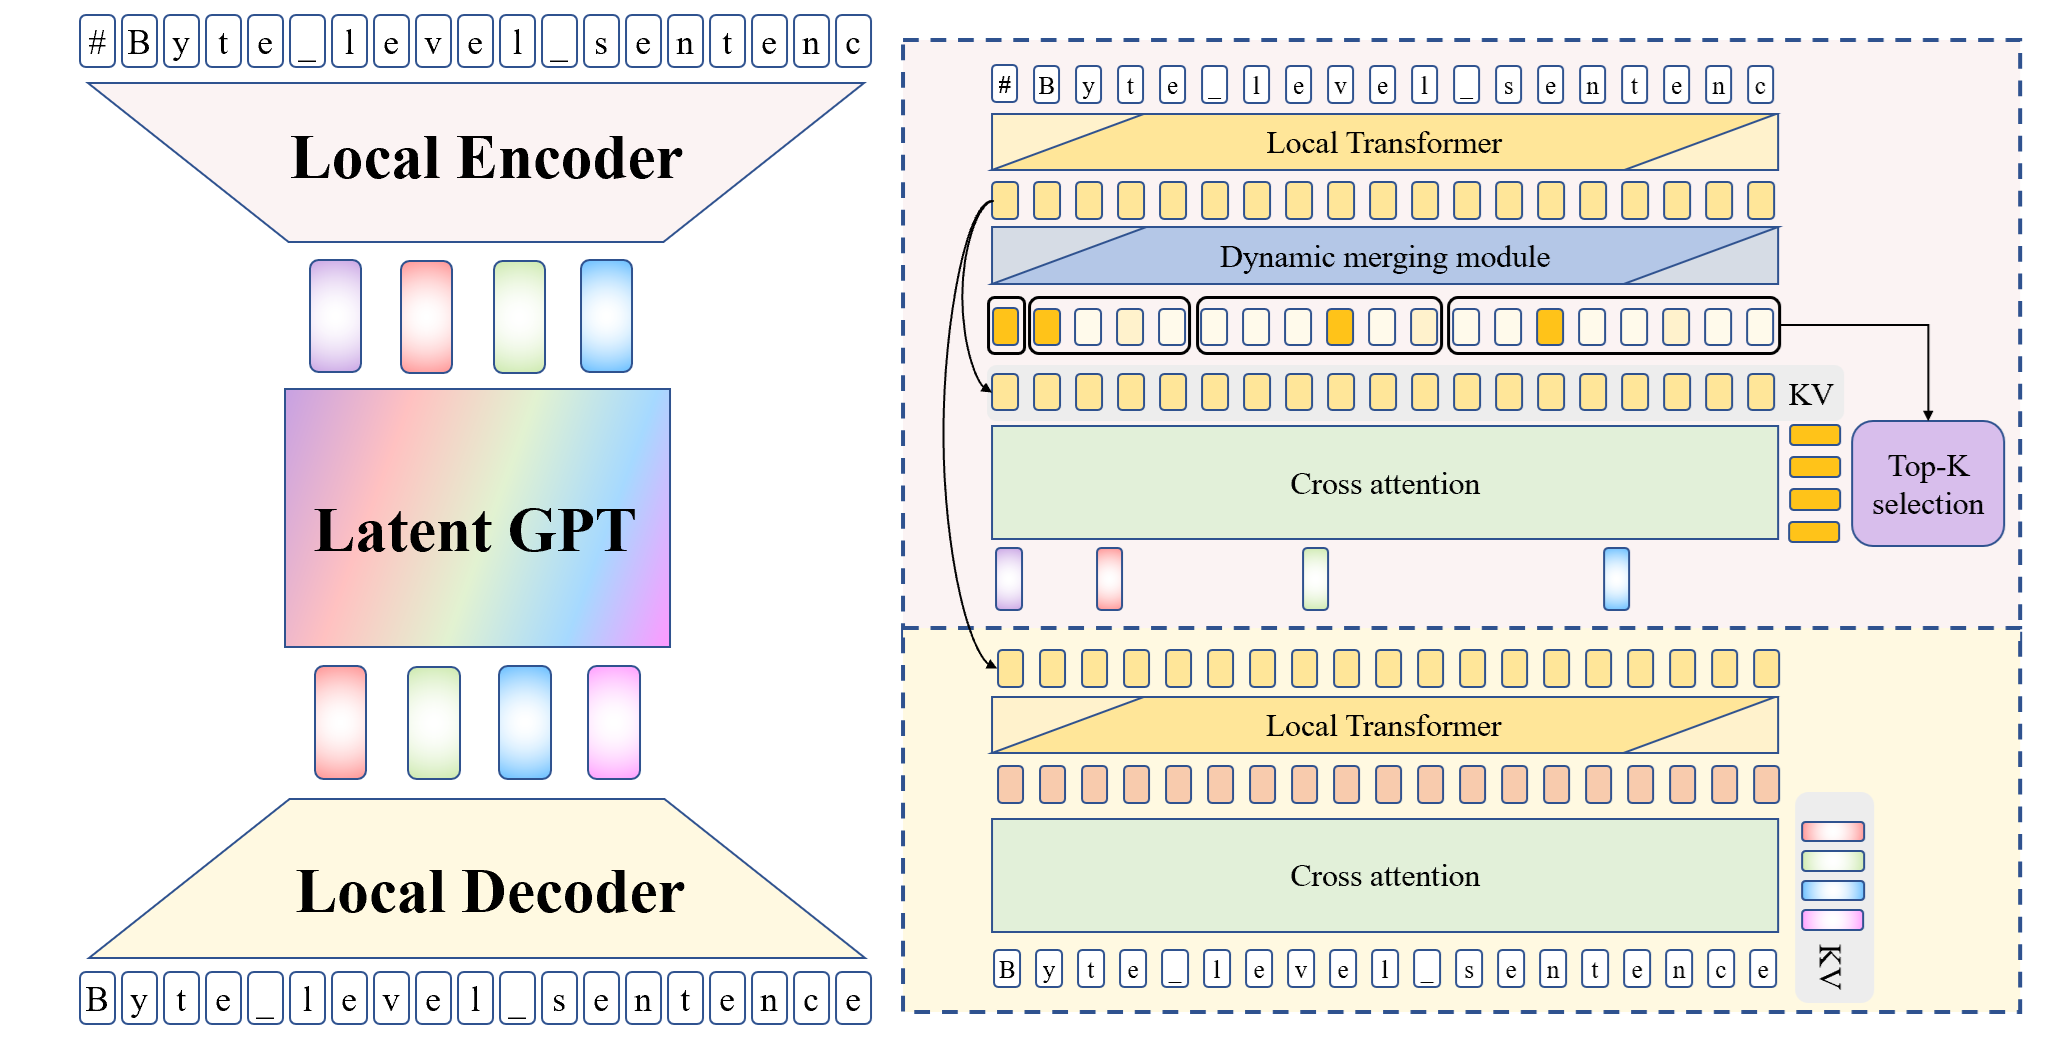
\includegraphics[width=1\linewidth]{模型.png}
    \caption{模型架构}
    \label{fig:placeholder}
\end{figure}
\subsection{LoE}
\subsubsection{LoT}

\textbf{角色：} 局部特征提取器。是整个架构的基石。其输出 $H$ 被复用于 Encoder 的压缩模块和 Decoder 的 Query 模块。

\begin{itemize}
    \item \textbf{输入：} $X$ + RoPE
    \item \textbf{结构：} $\#LoT$ 层 Transformer Block。
    \item \textbf{掩码：} Causal Mask $\in\mathbb{R}^{B\times L\times L}$。
    \item \textbf{每层输出：} $H_i \in \mathbb{R}^{B \times L \times d},\ \forall i\in \{1,\dots,\#LoT\}$
\end{itemize}

\subsubsection{可微令牌合并结构(共 $\#LoT$ 层)}
对于第 $i$ 层可微令牌合并结构：（为表述清晰，后续张量维度的推导与说明均以单一样本为准，默认隐去批次（Batch）维度 $B$。）
\begin{enumerate}
    \item 随机分组
\begin{itemize}
    \item 将当前序列索引随机划分为大小为 $N_a$ 的 Group A (Source) 和 大小为 $N_b$ 的 Group B (Target)。
    \item 状态变量：$H_a,H_b$ (Embeddings), $v_{i-1,a}, v_{i-1,b}$ (Mass), $S_{i-1,a}, S_{i-1,b}$ (Source Matrix)。在 OpenToMe 视觉实现中，metric 的输入可由 source trace 对每层 local block 输出做聚合；\texttt{center} 模式则只维护质心近似。
\end{itemize}
    \item  相似度与分配
    
计算 $A \rightarrow B$ 的相似度，经 SoftTopK 生成转移矩阵 $T_{ab} \in \mathbb{R}^{N_{a} \times N_{b}}$。
\item 双向更新

执行“质量转移”操作。Group B 吸收质量，Group A 扣除质量。

\begin{itemize}
    \item \textbf{Update Group B (Absorb):}
    \begin{align*}
        \text{Size: } & v_{i,b} = v_{i-1,b} + T_{ab}^{T}v_{i-1,a} \\
        \text{Source: } & {S}_{i,b} = S_{i-1,b} + \operatorname{Shift}_{a\rightarrow b}(T_{ab}, S_{i-1,a})
    \end{align*}

    \item \textbf{Update Group A (Decay):}
    Group A 将部分质量转移给 B 后，自身剩余的质量和来源记录需同步衰减。定义衰减系数向量 $d \in \mathbb{R}^{N_{a}}$ (即留存比例)：
    \begin{align*}
        d = 1 - T_{ab} 1_{N_{b}}\\
        v_{i,a} = v_{i-1,a} \odot d\\
        S_{i,a} = S_{i-1,a} \odot d
    \end{align*}
\end{itemize}
\end{enumerate}
\subsubsection{质心计算}

利用更新后的 Source Matrix 或轻量 center trace 计算每个 Token 在原始序列中的物理重心。这是后续时序排序的依据。

对于第 $i$ 个 Token：
    $c_{i} = \frac{\sum_{k=0}^{L-1} S_{i,k} \cdot k}{v_{i} + \epsilon}$
    $S_{i,k}$: Token $i$ 中来自原始位置 $k$ 的绝对贡献量，这边默认承认使用 $S_{\#LoT}$。若使用 \texttt{center} 模式，则直接维护 $c_i$ 而不显式保存 $S_{i,k}$。

\subsubsection{Downsampling \& Aggregation (Perceiver-style)}


\begin{itemize}
    \item \textbf{Top-N Selection (确定 Latent 原型):}
    根据 $v$ 选出质量最大的 $N$ 个索引。按质心 c 排序得到 $Idx_{sorted}$。
    
    \item \textbf{Perceiver Cross-Attention (生成 Z):}
    为表述严谨，我们先定义 $k_i$ 为第 $i$ 个 Latent Word 在原始 Byte 序列中的物理锚点索引：$k_i = Idx_{sorted}[i]$
    \begin{align}
        &\mathcal{Q}_{down} = H_{\#LoT}[Idx_{sorted}] + PosEmb_{latent} \\
        &K, V = H_{\#LoT} \\
        &Bias_{i,j} = \log(S_{\#LoT}[k_i, j] + \epsilon)
    \end{align}
    这个 source-aware bias 只对应完整 source matrix 路径；若采用轻量 center trace，则没有该项 source bias。OpenToMe 当前 CLS 分类路径还未消费 \texttt{token\_center}，因此 center 模式在该路径中应视作 dense source/bias off 的下界。
    
    \item \textbf{Operation:}
        $Z = \text{Softmax}\left(\frac{Q_{down}K^{T}}{\sqrt{d}} + Bias\right)V\in \mathbb{R}^{N \times d}$
\end{itemize}

\subsection{Latent Model (LaM)}
\begin{itemize}
    \item \textbf{结构：} Standard GPT (Decoder-only Transformer)。
    \item \textbf{输入：} Latent Words $Z$。
    \item \textbf{输出：} $O \in \mathbb{R}^{B \times N \times d}$，$O_{t}$ 为预测 $Z_{t+1}$ 的语义信息。
\end{itemize}

\subsection{Local Decoder (LoD)}
\textbf{角色：} 连续上采样解码器。

\begin{itemize}
    \item \textbf{Q Source:} 直接复用 LoT 输出 $H_{\#LoT}$。
    \item 物理意义：$H_{t}$ 聚合了 $L_{1 \dots t}$ 的上下文。
    \item \textbf{KV Source:}
    \begin{itemize}
        \item Training: $Z$ (Phase 1) 或 $O$ (Phase 2)。
        \item Inference: Latent Queue $\mathcal{Q}$。
    \end{itemize}
    
    \item \textbf{Cross-Attention Mechanism (With Band Mask):}
    为了对齐推理时的滑动窗口限制，训练时需施加 Band Mask，模拟有限视场。
    \begin{equation*}
        AttnScore_{t,j} = \frac{Q_{t}K_{j}^{T}}{\sqrt{d}} + Bias_{grid}(t,j) + M_{band}(t,j)
    \end{equation*}
    
    \item \textbf{Relative Grid Bias:}
    \begin{equation*}
        Bias_{grid} = -\gamma \cdot \left|\frac{t}{\lambda} - j\right|
    \end{equation*}
    (起到类似位置编码的作用，引导模型关注逻辑位置相近的 Latent Words)
    
    \item \textbf{Causal Mask:}
    (这强制训练时的模型也只能看到局部窗口往前的 Latent Words，与推理时的 Queue 保持一致)
    \begin{equation*}
        M_{causal}(t,j) = \begin{cases} 
            0 & \text{if } 0 \le (\lceil t/\lambda \rceil - j) < W_{infer} \\ 
            -\infty & \text{otherwise} 
        \end{cases}
    \end{equation*}
\end{itemize}

\section{生成过程}

\textbf{核心定义}
\begin{itemize}
    \item $W_{infer}$: 滑动窗口大小。
    \item $\mathcal{Q}$: 队列，长度维持在 $W_{infer}$。
    \item $ptr$: 当前 Byte 指针。
\end{itemize}

\textbf{1. Initialization (Start)}
\begin{itemize}
    \item \textbf{Context:} [BOS] + prompt
    \item 通过 LoT, LoE 得到输出 $z=[z_{1}, z_{2}, \dots, z_{L}]$
    \item LaM 接收 $z$ 输出 word 序列 $o=[o_{1}, o_{2}, \dots, o_{L}]$ ($o_{L}$ 在预测 $z_{L+1}$)
    \item 初始化队列：$\mathcal{Q}=[o_{L-W_{infer}+1}, \dots, o_{L}]$ (如果有不合法位置 pad 为 0)。
    \item $ptr$ 初始化为 $L$。
\end{itemize}

\textbf{2. Generation Loop}
循环直到采样到 [EOS]:
\begin{itemize}
    \item \textbf{Byte Generation:}
    \begin{itemize}
        \item LoD 利用队列 $\mathcal{Q}$ 进行解码 (Cross Attn) 生成 Byte: $b_{new} = LoD(Context, \mathcal{Q}, ptr)$
        \item 滑动指针 $ptr \leftarrow ptr + 1/\lambda$，将 $b_{new}$ 加入 context 末尾。
        \item 如果 $\lfloor ptr \rfloor$ 发生变化，我们认为应该进行下一个词：
        \item $\mathcal{Q}.\text{pop\_front}()$ (丢弃最老的历史)
        \item 使用 LaM 自回归生成 $o_{next}$
        \item $\mathcal{Q}.\text{push\_back}(o_{next})$ (将新预测加入队尾)
        \item 状态：队列变为 $[\dots, o_{L}, o_{next}]$，准备生成下一段 Bytes。
    \end{itemize}
\end{itemize}

\end{document}
